\chapter{Classificazione}
\label{chapter:classification}

Il cuore del progetto riguarda la classificazione delle attività mediante i dati ottenuti.

Ho optato per l'utilizzo di Keras per l'implementazione della rete neurale di cui vediamo le 
fasi di \textit{training} e di \textit{prediction}.
\subsubsection{Keras}
Keras \cite{keras} è una libreria open-source per le reti neurali che astrae lo sviluppo rendendolo più comprensibile, 
pur mantenendo pieno supporto alle librerie di più basso livello (es. Tensorflow \cite{tensorflow}) su cui si basa.



\section{Apprendimento e Test}
Un classificatore basa le sue predizioni sui modelli che riesce a ricavare dall'insieme di informazioni che ha a disposizione.
Nel nostro caso l'insieme di queste informazioni è contenuto nei file CSV nei quali è salvato lo storico di tutti 
i dati ricevuti dall'applicazione.


\subsection{Caricamento dei dati}
I file CSV sono organizzati come nell'esempio visto in figura \ref{fig:example-dataset-csv-accelerometer}.

\vspace{5mm} %5mm vertical space

È necessario ricordare che i dati ottenuti da differenti sensori sono stati immagazzinati dal \textit{modulo di comunicazione} in diversi file CSV. 
Nel caso in esame sono quindi presenti due file, uno per l'accelerometro ed un secondo per il giroscopio.

\vspace{5mm} %5mm vertical space

Entrambi contengono la stessa tipologia di informazioni e sono strutturati in modo equivalente.
Per semplificare la trattazione nelle procedure seguenti sarà considerato un singolo dataset, ricordando però di dover applicare tutti i 
passaggi indistintamente ad entrambi.

\subsubsection{Lettura del file}
L'intero dataset contiene un ampio numero di record, ognuno dei quali è composto dalle seguenti informazioni:
\begin{itemize}
    \item un identificativo che raggruppa i valori ottenuti da una singola esecuzione
    \item un indice crescente che ordina i record di un archivio
    \item i valori acquisiti dal sensore
    \item l'istante temporale di acquisizione
    \item la posizione del dispositivo
    \item la relativa attività
\end{itemize}
Come si può notare i valori contenuti in un record hanno corrispondenza $1:1$ con quelli 
inviati dall'applicazione in un singolo messaggio durante l'apprendimento. L'unica eccezione è 
il relativo tipo di sensore, già utilizzato per la divisione preliminare.

\begin{listing}[H] 
    \inputminted[frame=single,framesep=10pt]{python}{assets/snippets/classifier/read_csv.py}
    \caption{Creazione del dataframe a partire dal file CSV}
\end{listing}


\subsection{Valutazione della posizione del dispositivo}
Comunemente durante lo sviluppo di tecniche per il riconoscimento delle attività la posizione del dispositivo di 
raccolta dati viene spesso sottovalutata. Tuttavia si tratta di un aspetto molto importante per 
una miglior classificazione \cite{umafall}.

\vspace{5mm} %5mm vertical space

Dopo una prima valutazione che prevedeva l'utilizzo di questo dato come una semplice caratteristica informativa, ho deciso 
di dare ad esso un'importanza maggiore. 

Il maggior valore è derivato dalla decisione di partizionare nuovamente i record presenti nel dataset in base alla relativa posizione. 
Tale scelta comporta la necessità di eseguire le procedure di \textit{train} e \textit{test} seguenti su tutte 
le diverse partizioni e conseguentemente la creazione di un modello indipendente per ognuna di esse.

\vspace{5mm} %5mm vertical space

Ai fini della trattazione proseguirò considerando solamente il gruppo di dati relativo ad una posizione 
tra quelle che ho personalmente impostato.

Ricordando che i dati sono già stati in precedenza partizionati in base al sensore di riferimento, è importante tener presente 
che tutte le seguenti procedure dovranno essere ripetute per ogni posizione e per ogni sensore.

\vspace{5mm} %5mm vertical space

Consideriamo quindi solo i dati \textit{accelerometrici} e \textit{"nella mano destra"}.


\subsection{Visualizzazione grafica dei dati}
\subsubsection{Suddivisione grafica}
Per ogni partizione di dati che si va a considerare è possibile ottenere una chiara visualizzazione grafica 
della suddivisione per attività dei dati presenti.
\begin{figure}[H]
    \centering
    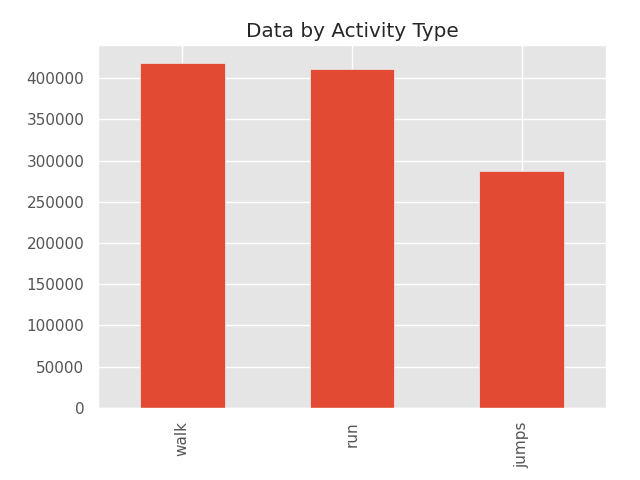
\includegraphics[scale = 0.60]{assets/images/classifications/accelerometer/right_hand/activity-type-graph-right-hand-acc.png}
    \caption{Visualizzazione della suddivisione per attività}
\end{figure}

\subsubsection{Grafici delle attività}
Per ogni attività è inoltre possibile ottenere una visualizzazione grafica. Questi grafici ci permettono di comprendere meglio le differenze 
tra le varie attività sulla base dei valori inerziali ottenuti senza dover analizzare matematicamente i valori.

\begin{figure}[H]
    \centering
    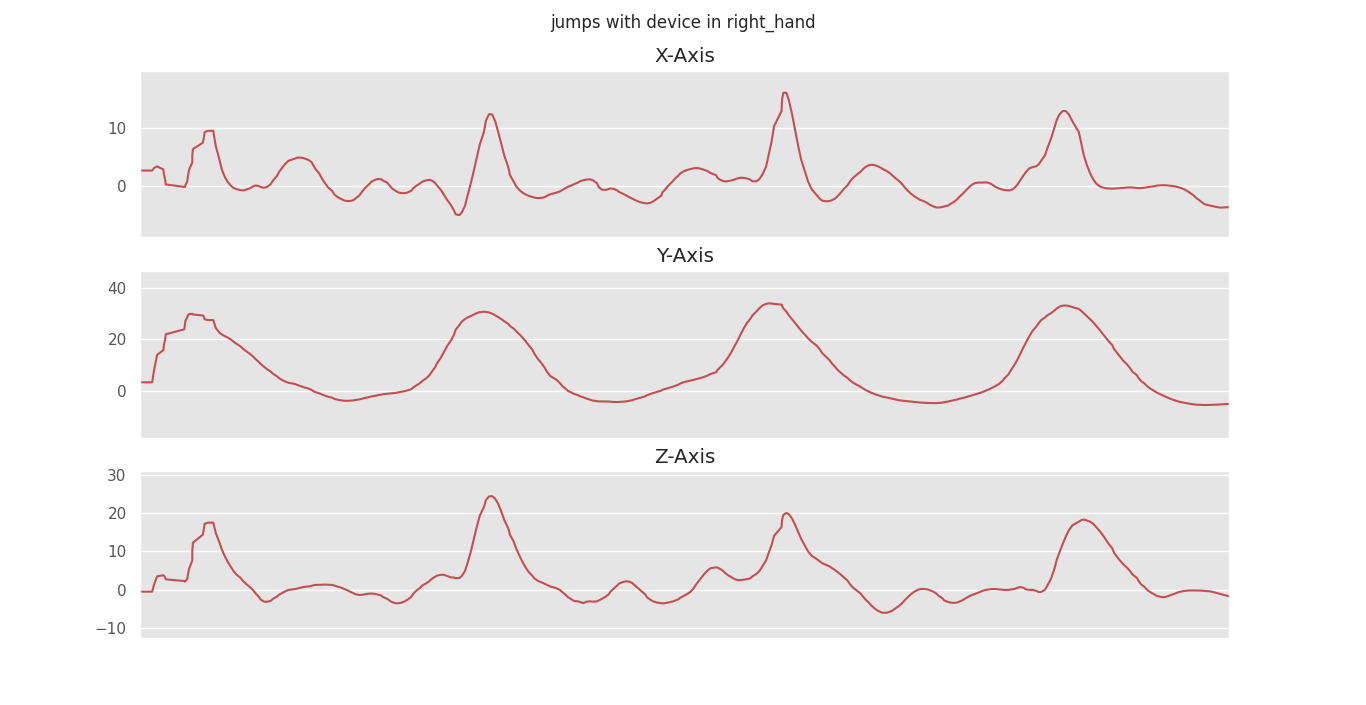
\includegraphics[scale = 0.45]{assets/images/classifications/accelerometer/right_hand/jumps-right-hand-acc.png}
    \caption{Dati accelerometrici durante l'attività "Salti"}
\end{figure}
\begin{figure}[H]
    \centering
    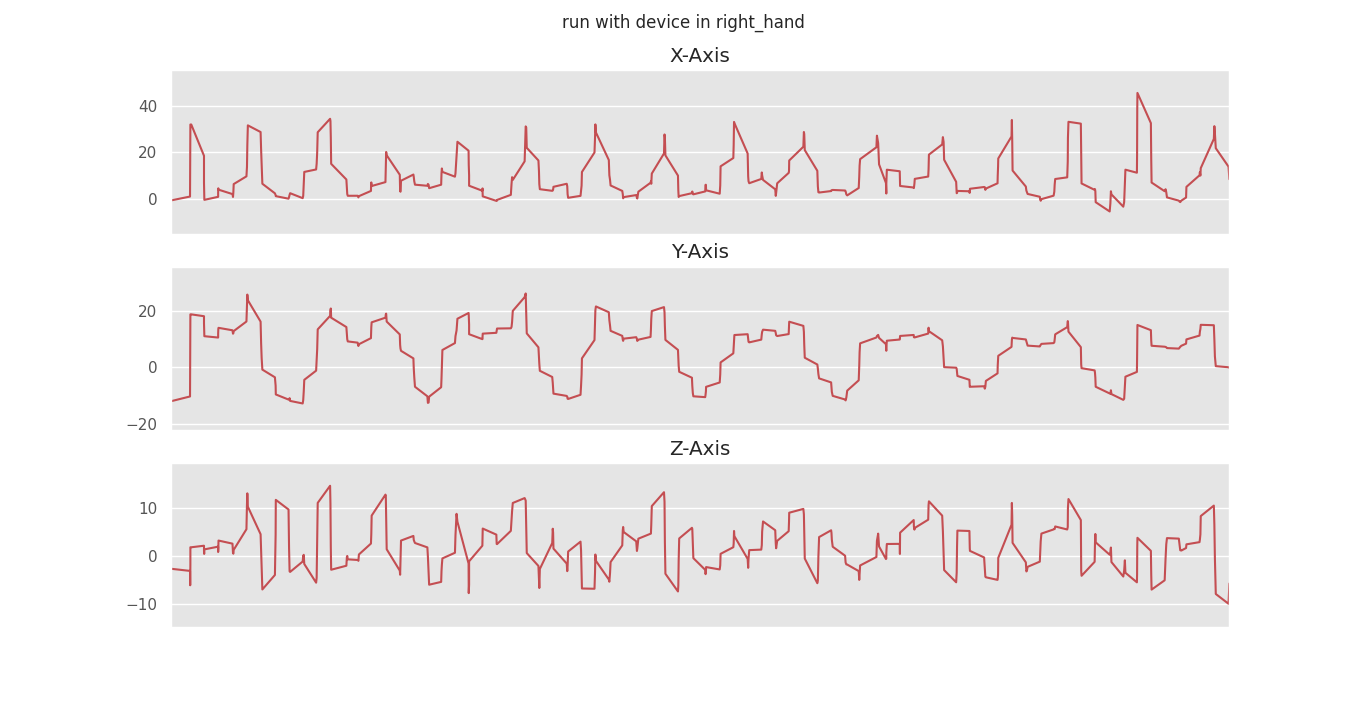
\includegraphics[scale = 0.45]{assets/images/classifications/accelerometer/right_hand/run-right-hand-acc.png}
    \caption{Dati accelerometrici durante l'attività "Corsa"}
\end{figure}
\begin{figure}[H]
    \centering
    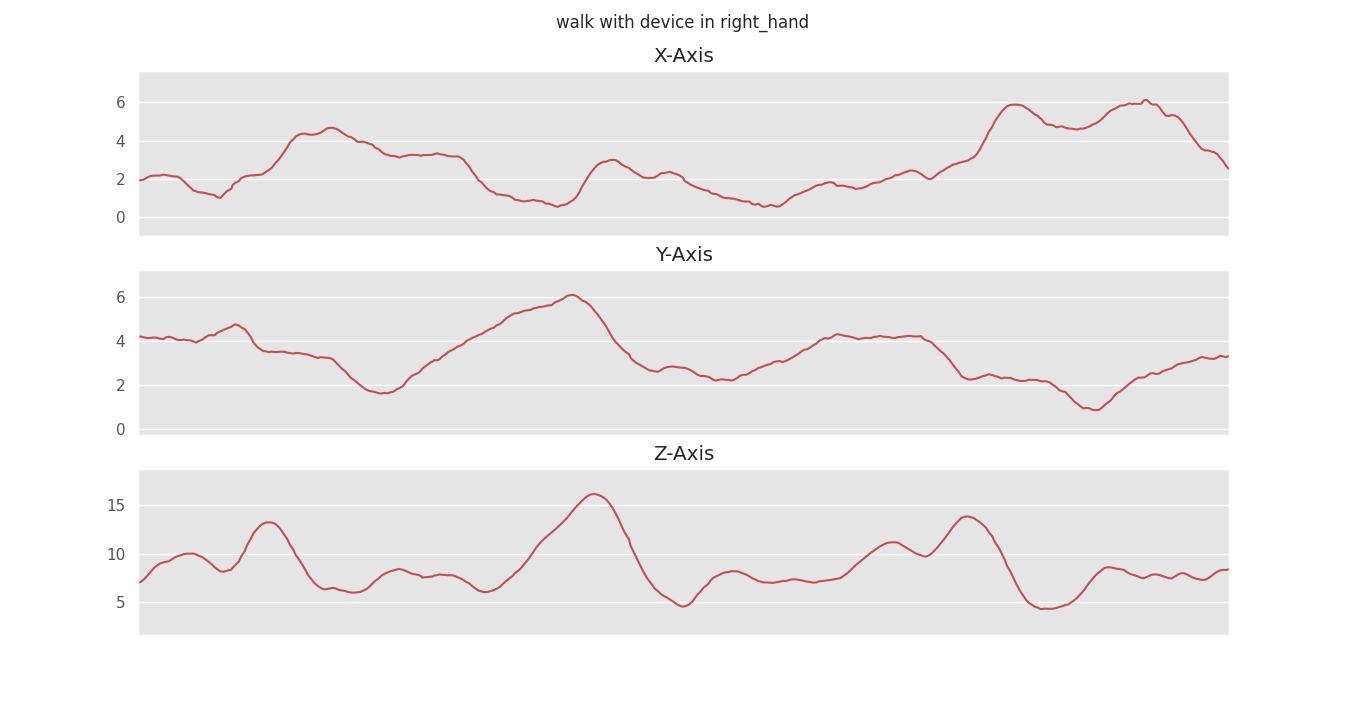
\includegraphics[scale = 0.45]{assets/images/classifications/accelerometer/right_hand/walk-right-hand-acc.png}
    \caption{Dati accelerometrici durante l'attività "Camminata"}
\end{figure}


\newpage
\subsection{Partizionamento dei dati}
La mole di dati considerata necessita un ulteriore partizionamento per differenziare i dati che saranno utilizzati per 
l'\textit{apprendimento} e quelli che saranno utilizzati per il \textit{test}.

È indispensabile verificare che le partizioni non abbiano sovrapposizioni se non si vuole ottenere una valutazione dell'efficienza falsata.

\vspace{5mm} %5mm vertical space

Personalmente ho scelto una semplice suddivisione che prevede l'utilizzo di $\frac{4}{5}$ dei dati per il \textit{train} e 
la parte restante ($\frac{1}{5}$) per il \textit{test}.


\subsection{Preparazione dei dati}
\label{section:learning-data-preparation}
A questo punto è necessario organizzare i dati in nostro possesso in modo che 
ad una serie di caratteristiche (i tre assi x, y, z ed il valore temporale) sia associabile un'etichetta 
rappresentate l'attività. 

\subsubsection{Trasformazione del valore temporale}
Una delle quattro caratteristiche che intendiamo utilizzare è il valore temporale.

I file CSV contenevano però i \textit{timestamp}s che rappresentano il tempo assoluto, 
ovvero il momento esatto di svolgimento dell'attività durante la raccolta dei dati.
Questo valore non è in alcun modo rilevante nella classificazione, ma a partire da esso è possibile ricavare il tempo trascorso 
tra l'acquisizione di una tripla di dati (x, y, z) e l'acquisizione di quella immediatamente successiva.
Posso presumere una somiglianza in tali distanze temporali durante lo svolgimento di una uguale attività.

\subsubsection{Normalizzazione dei dati}
La rete neurale accetta in ingresso valori compresi tra 0 e 1. Eseguo quindi anche una semplice normalizzazione delle caratteristiche.
\begin{listing}[H] 
    \inputminted[frame=single,framesep=10pt]{python}{assets/snippets/classifier/normalize_data.py}
    \caption{Banale normalizzazione dei dati}
\end{listing}

\newpage
\subsubsection{Creazione dei segmenti e delle etichette}
La parte principale dell'intero adattamento risulta essere quella che suddivide i dati in un formato che possa 
realizzare l'associazione tra una serie di caratteristiche e una etichetta.

Per realizzare ciò i record sono presi a gruppi, anche sovrapposti (così come si vede in figura \ref{fig:create_segments_and_labels}). 
Ogni raggruppamento sarà caratterizzato da 
\begin{itemize}
    \item una finestra di record contenenti le sole caratteristiche
    \item l'etichetta più frequente
\end{itemize}

\begin{figure}[H]
  \centering
  \includesvg[scale = 0.70]{assets/graphs/create_segments_and_labels.svg}
  \caption{Creazione delle finestre e delle etichette}
  \label{fig:create_segments_and_labels}
\end{figure}

\begin{figure}[H]
  \centering
  \includesvg[scale = 1.0]{assets/graphs/segments_and_labels.svg}
  \caption{Risultato dopo la creazione delle finestre e delle etichette}
  \label{fig:segments_and_labels}
\end{figure}

Alla fine del processo ho quindi ottenuto una serie di finestre di dati a cui posso singolarmente associare una determinata
etichetta identificativa.

\subsubsection{Ampiezza delle finestre}
Ho implementato una finestra di caratteristiche capace di contenere $80$ record. Ricordando la frequenza di 
campionamento dei sensori di $f_c = 20$ Hz e il relativo periodo di campionamento di $T_c = 50ms = 0.5s$, ogni finestra rappresenta i dati ottenuti in 
$$T_f = 0.5s * 80 = 4s$$

\subsubsection{Sovrapposizione delle finestre}
Durante la lettura di tutti i record da convertire, la finestra scorre in avanti di $40$ passi alla volta.

Essendo $40$ inferiore alla dimensione scelta per l'ampiezza della finestra ($80$), si genera una sovrapposizione (\textit{overlap}).
Perciò la quasi totalità dei record (ad eccezione di quelli agli estremi) comparirà in 2 finestre distinte.

\begin{listing}[H] 
    \inputminted[frame=single,framesep=10pt]{python}{assets/snippets/classifier/create_segments_and_labels.py}
    \caption{Creazione delle finestre e delle etichette}
\end{listing}


\newpage
\subsection{Creazione della rete neurale}
Una volta generati i dati nel formato supportato da \textit{keras} procedo alla creazione di 
una rete neurale che abbia
\begin{itemize}
    \item in input il formato dei dati appena generato
    \item 5 strati di 100 nodi connessi
    \item in output il calcolo di probabilità per ogni classe
\end{itemize}
\begin{listing}[H] 
    \inputminted[frame=single,framesep=10pt]{python}{assets/snippets/classifier/dnn_create.py}
    \caption{Creazione della rete neurale}
\end{listing}
Per poi procedere all'apprendimento.
\begin{listing}[H] 
    \inputminted[frame=single,framesep=10pt]{python}{assets/snippets/classifier/dnn_fit.py}
    \caption{Apprendimento della rete neurale}
\end{listing}


\newpage
\subsection{Statistiche del modello}
Al termine dell'attività di apprendimento il modello è stato generato. Ed è possibile vedere un grafico 
riassuntivo dei risultati ottenuti.
\begin{figure}[H]
    \centering
    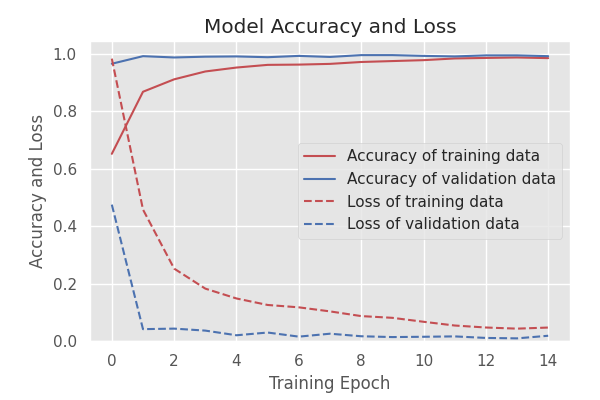
\includegraphics[scale = 0.60]{assets/images/classifications/accelerometer/right_hand/model-right-hand-acc.png}
    \caption{Statistiche del modello ottenuto}
\end{figure}


\subsection{Salvataggio del modello}
Il modello generato è facilmente salvato in un file con estensione \textit{.h5} che mi permetterà in seguito 
di ricaricarlo senza dover rieffettuare l'intero processo sui dati.
\begin{listing}[H] 
    \inputminted[frame=single,framesep=10pt]{python}{assets/snippets/classifier/save_model.py}
    \caption{Salvataggio del modello ottenuto}
\end{listing}


\subsection{Testing della rete neurale}
Per testare il modello appena creato utilizzo la partizione precedentemente separata.

L'intento è quello di effettuare una predizione con i dati di test di cui però si conoscono già i risultati. 
Sarà quindi immediato trovare l'efficienza del modello creato mediante un banale confronto tra i dati ipotizzati 
dalla rete neurale e i risultati corretti.

La qualità dei dati può essere visualizzata mediante una \textit{matrice di confusione} che fornisce una rappresentazione 
grafica del confronto appena descritto.

\subsubsection{Matrice di confusione}
La matrice di confusione è una tabella di rappresentazione dell'accuratezza di un modello di classificazione. 
In una matrice di confusione sono contrapposti i valori ipotizzati da un modello di classificazione e i valori reali 
di cui si conosceva il corretto risultato.

\begin{figure}[H]
    \centering
    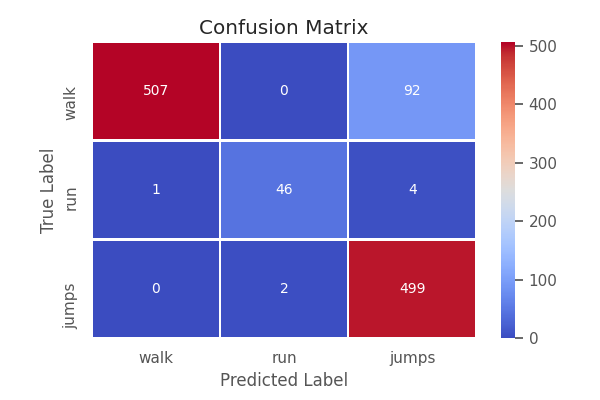
\includegraphics[scale = 0.70]{assets/images/classifications/accelerometer/right_hand/confusion-matrix-right-hand-acc.png}
    \caption{Matrice di confusione del modello ottenuto}
\end{figure}


\section{Predizioni}
Il processo di predizione consiste nell'ipotizzare, grazie ad un modello tra quelli generati, 
l'etichetta più opportuna da assegnare ad un insieme di record contenenti
\begin{itemize}
    \item i valori ottenuti dal sensore
    \item il dato temporale
    \item il tipo di sensore a cui si riferiscono
    \item la posizione del dispositivo durante l'esecuzione
\end{itemize}


\subsection{Scelta del modello}
Per prima cosa, tra le informazioni devo differenziare i dati che mi permetteranno di identificare il modello e le caratteristiche 
su cui avvierò la predizione.

Ricordo che durante l'apprendimento l'informazione che identificava il tipo di sensore e quella che differenziava 
la posizione del dispositivo sono state utilizzate per la generazione di differenti modelli.
Disponendo di queste informazioni è quindi possibile ricavare il modello corretto.

Si nota che le informazioni rimanenti (valori degli assi e valore temporale) corrispondono alle caratteristiche di analisi.


\subsection{Preparazione dei dati}
Fornita una serie di caratteristiche (i tre assi x, y, z ed il valore temporale), ci si aspetta di ottenere 
in risposta un'etichetta rappresentante l'attività.

\vspace{5mm} %5mm vertical space

Perchè tutto funzioni è indispensabile che i dati forniti alla rete neurale durante la fase di ipotesi 
abbiano la stessa struttura di quelli utilizzati durante la generazione dei modelli.
Si attuano in questa fase le stesse procedure viste in precedenza nella corrispondente sezione 
\ref{section:learning-data-preparation} di apprendimento.

\subsubsection{Operazioni preliminari}
Per prima cosa si attua la trasformazione del valore temporale dal significato assoluto a quello relativo.
Ed in seguito si normalizzano le 4 caratteristiche.


\subsubsection{Creazione dei segmenti}
L'insieme dei record è nuovamente preso a gruppi, anche sovrapposti, per la creazione dei segmenti.

\begin{figure}[H]
    \centering
    \includesvg[scale = 0.75]{assets/graphs/create_segments.svg}
    \caption{Creazione dei segmenti}
    \label{fig:create_segments}
\end{figure}

\begin{figure}[H]
    \centering
    \includesvg[scale = 1.0]{assets/graphs/segments.svg}
    \caption{Risultato dopo la creazione dei segmenti}
    \label{fig:segments}
\end{figure}



\subsection{Ipotesi dell'etichetta}
A questo punto il lavoro è delegato alla rete neurale che ricevendo in input l'insieme dei segmenti 
e con l'ausilio del modello selezionato fornisce in output l'insieme delle etichette ipotizzate.
Il risultato ottenuto è un'insieme di etichette, ognuna associata ad un segmento. 

Per ricavare l'etichetta assoluta associata alle caratteristiche date in input procedo banalmente 
considerando quella che compare più volte.

\begin{figure}[H]
    \centering
    \includesvg[scale = 1.0]{assets/graphs/prediction.svg}
    \caption{Processo di predizione}
    \label{fig:prediction}
\end{figure}
